%!TEX program = xelatex
%!TEX options = --shell-escape

\documentclass[10pt, aspectratio=169]{beamer}

\usetheme{oxford}
\usefonttheme[onlymath]{serif}

\setsansfont{FoundrySterling-Book}[
  BoldFont=FoundrySterling-Bold,
  ItalicFont = FoundrySterling-BookItalic
]

\usepackage{minted}
\usepackage{booktabs}
\usepackage{array}
\usepackage{ragged2e}
\usepackage[os=win]{menukeys}

\title{A few bits of Unix}
\date{\scriptsize \today}
\author{Nicolas Payette}
\institute{%
  
\includegraphics[height=15mm]{img/cohesys_logo_light_oxford}
}

\usepackage{listings}
\lstset{basicstyle=\ttfamily\bfseries\color{OxfordBlue}}
\let\cmd=\lstinline

\newcommand{\cmdit}[1]{\textit{\hl{#1}}}
\newcommand{\tgu}[1]{\tiny\textcolor{gray}{\url{#1}}}

\begin{document}

\maketitle

\begin{frame}[fragile]
  \begin{columns}[T]
    \begin{column}{0.75\textwidth}
      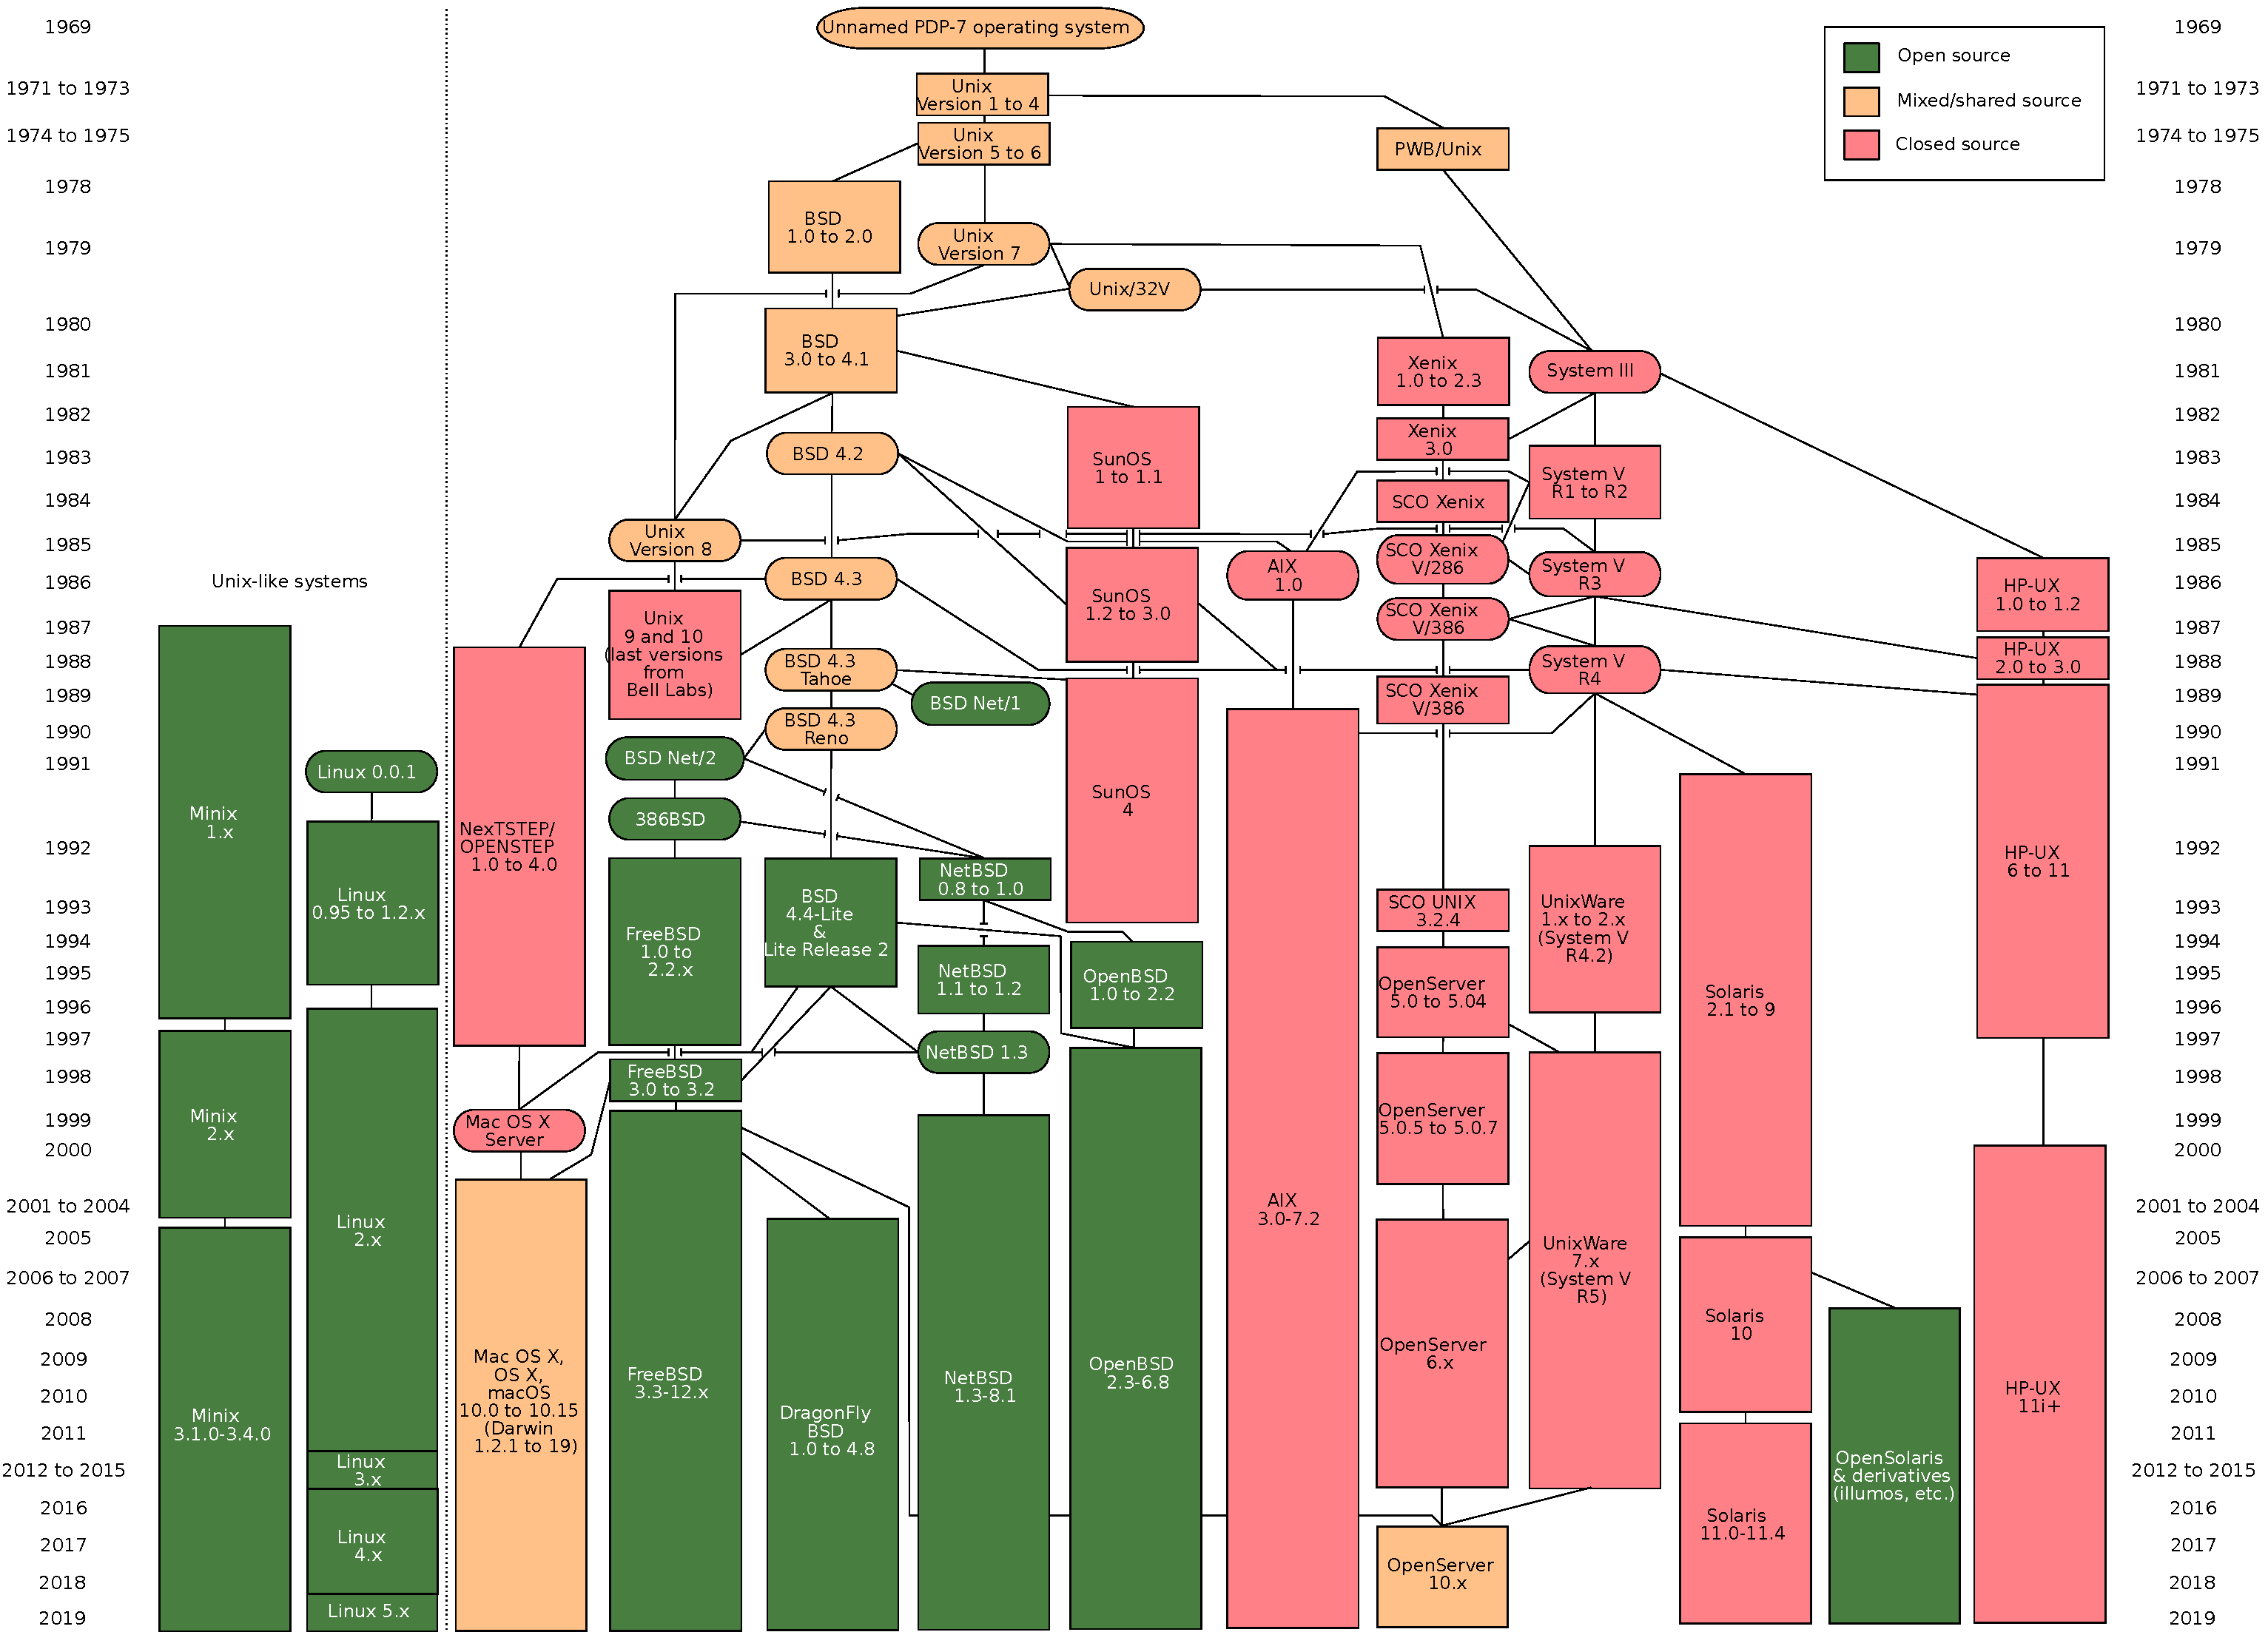
\includegraphics[height=0.85\textheight]{img/unix_history.pdf}\\[1mm]
      \tiny\textcolor{gray}{\url{https://w.wiki/_zu2j}}
    \end{column}
    \begin{column}{0.25\textwidth}
      \hl{Linux} is the most popular Unix derivative.
      \vskip5mm
      \hl{macOS} is a proper Unix system.
      \vskip5mm
      \hl{Android} runs on\\a Linux kernel.
      \vskip5mm
      Even \hl{Windows} is relenting, nowadays:\\[2mm]\tiny
      \url{https://docs.microsoft.com/en-us/windows/wsl/about}
    \end{column}
  \end{columns}

\end{frame}

\begin{frame}[fragile]
  \vfill
  \begin{tabular}{%
    >{\RaggedRight\arraybackslash}p{0.15\textwidth}%
    >{\RaggedRight\arraybackslash}p{0.15\textwidth}%
    >{\RaggedRight\arraybackslash}p{0.15\textwidth}%
    >{\RaggedRight\arraybackslash}p{0.15\textwidth}%
    >{\RaggedRight\arraybackslash}p{0.15\textwidth}%
  }
    \hl{Unix} &
    \hl{GNU} &
    \hl{Linux} &
    \hl{Ubuntu} &
    \hl{Bash} \\    
    \addlinespace[2mm]
    A family of operating systems &
    A collection of free Unix-like tools (``GNU's Not Unix!") &
    An open-source Unix-like kernel &
    A GNU/Linux distribution &
    A shell and command language (``Bourne Again SHell'') \\
    \addlinespace[8mm]
    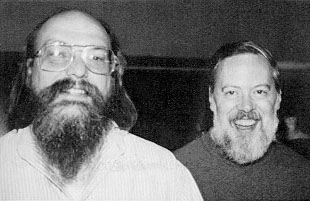
\includegraphics[height=0.175\textheight]{img/thompson_and_ritchie.jpg} &
    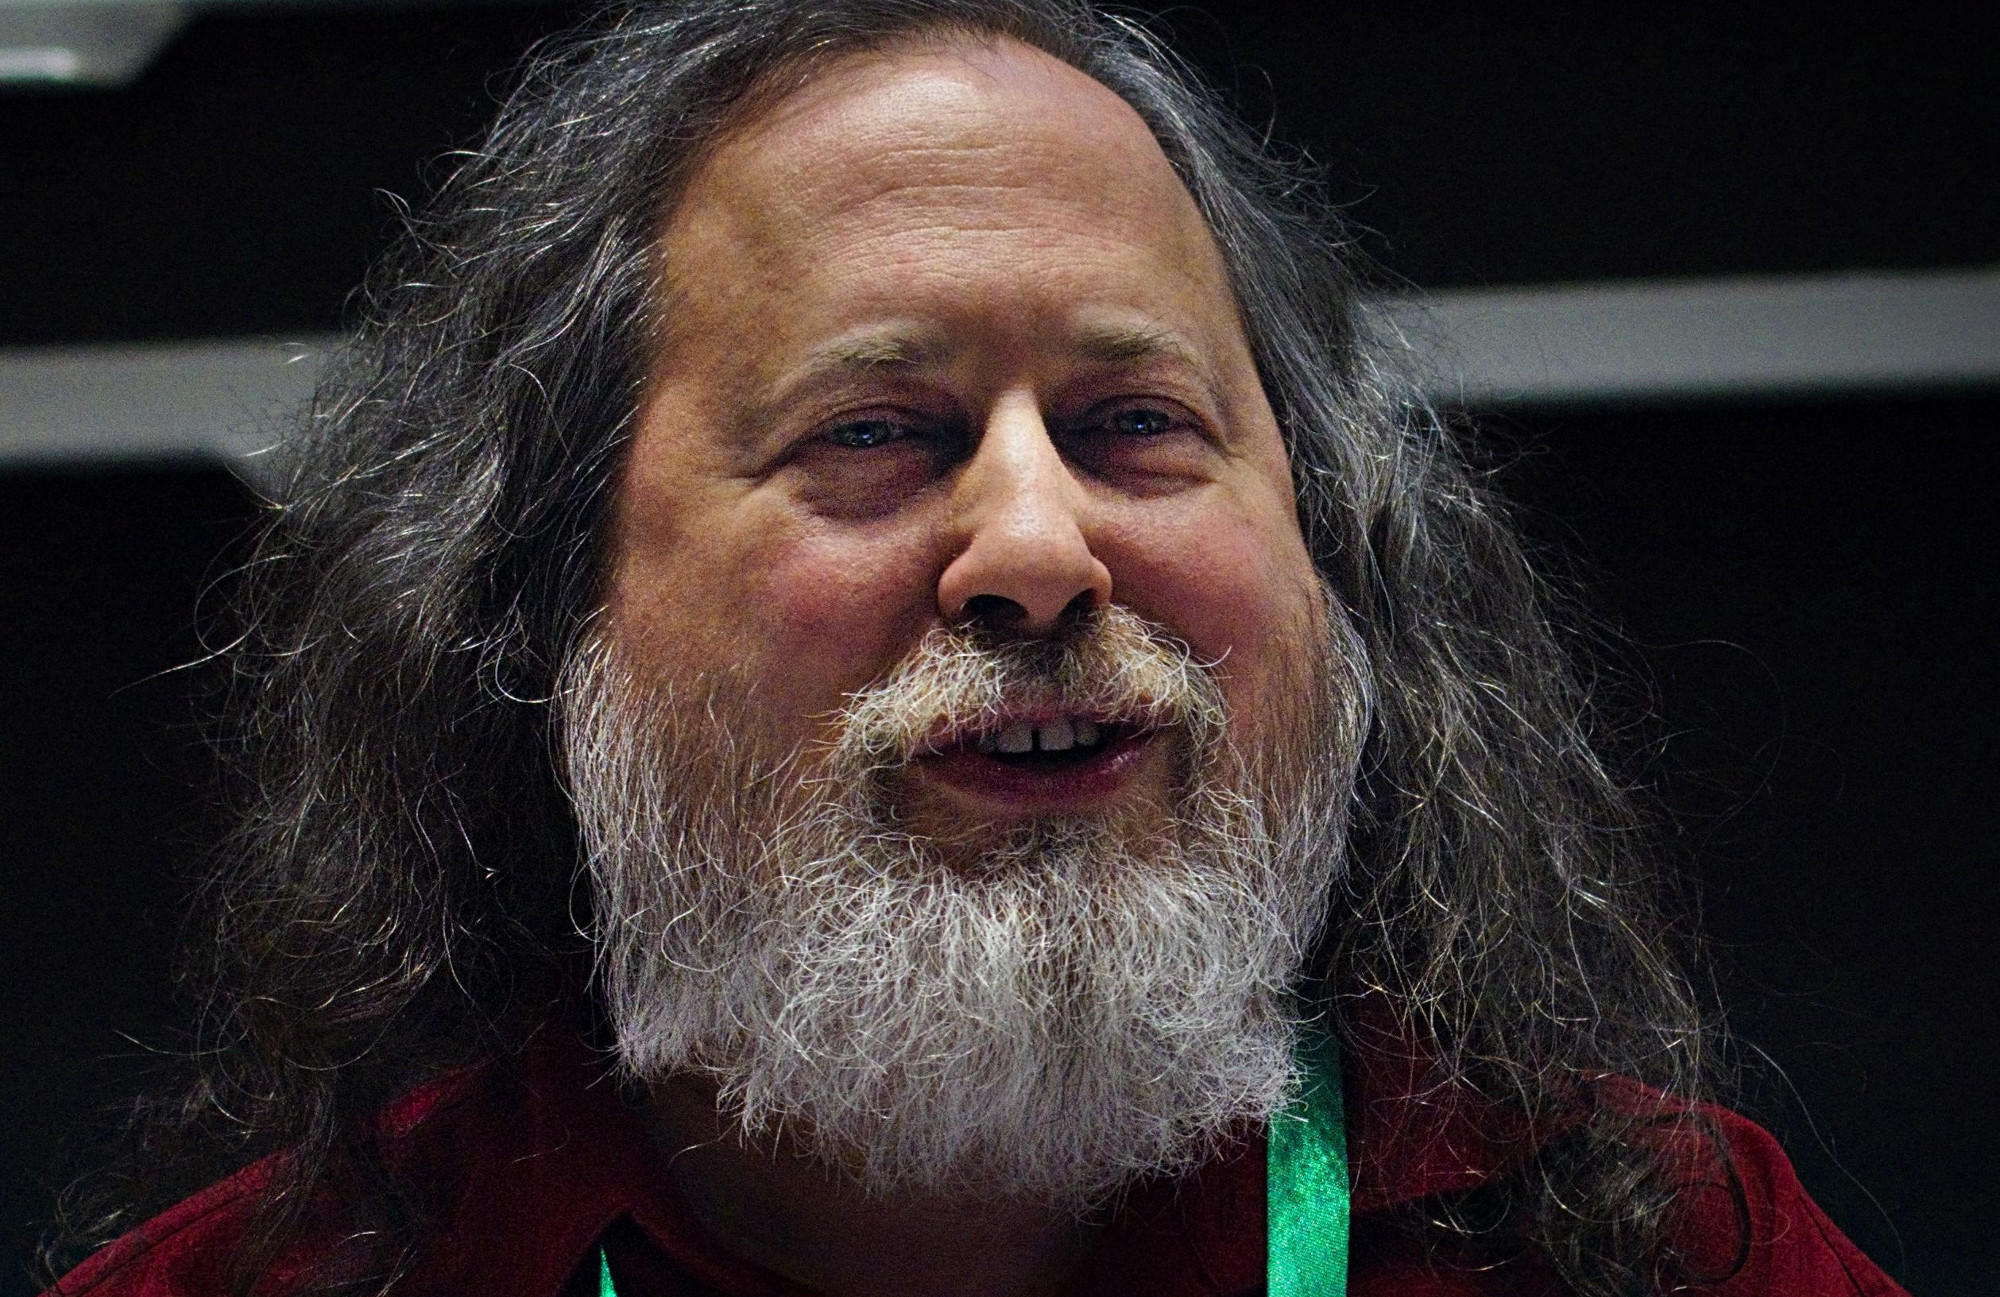
\includegraphics[height=0.175\textheight]{img/stallman.jpg} &
    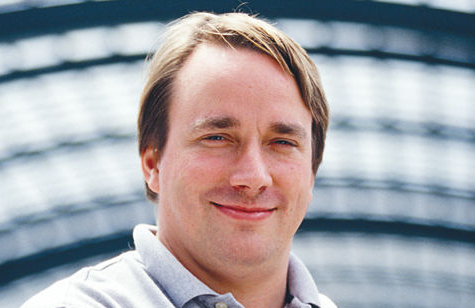
\includegraphics[height=0.175\textheight]{img/torvalds.jpeg} &
    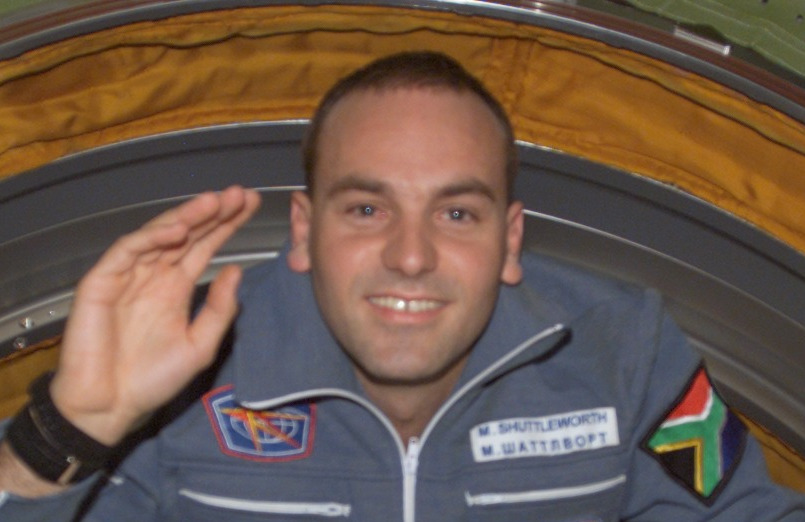
\includegraphics[height=0.175\textheight]{img/shuttleworth.jpg} &
    \includegraphics[height=0.175\textheight]{img/fox.png} \\
    \tgu{https://w.wiki/392t} &
    \tgu{https://w.wiki/392w} &
    \tgu{https://w.wiki/392v} &
    \tgu{https://w.wiki/392y} &
    \tgu{https://w.wiki/392$} \\
  \end{tabular}
  \vfill
\end{frame}

\begin{frame}{The Unix philosophy}
  \begin{columns}
    \begin{column}{0.65\textwidth}
      \LARGE
      \begin{itemize}
        \item Write programs that do one thing and do it well.
        \vskip5mm
        \item Write programs to work together.
        \vskip5mm
        \item Write programs to handle text streams, because that is a universal interface.
      \end{itemize}
    \end{column}
    \begin{column}{0.35\textwidth}
      \tiny
      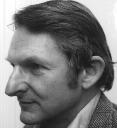
\includegraphics{img/doug.jpg}\\[1mm]
      \textcolor{gray}{\url{https://www.cs.dartmouth.edu/~doug/}}
      \\[1cm]
      \hl{Doug McIlroy}, as quoted in Peter H. Salus. \emph{A Quarter-Century of Unix}. Addison-Wesley. 1994. ISBN 0-201-54777-5.
    \end{column}
  \end{columns}
\end{frame}

\begin{frame}
  \vfill
  {\huge\cmd{ls}\quad list directory contents}
  \vfill
  Useful options:\\[2mm]
  \begin{itemize}
    \item \cmd{ls -a}, \cmd{--all}\quad do not ignore entries starting with a dot
    \item \cmd{ls -l}\quad use a long listing format
    \item \cmd{ls -h}, \cmd{--human-readable}\quad print sizes like \texttt{1K}, \texttt{234M}, \texttt{2G}, etc.
    \item \cmd{ls -1}\quad list one file per line
    \item \cmd{ls -S}\quad sort by size, largest first
  \end{itemize}
  \vfill
  And more! To find out, use: \cmd{man ls}.
\end{frame}

\begin{frame}
  \vfill
  {\huge\cmd{cd}\quad change directory}
  \vfill
  \begin{itemize}
    \item \cmd{cd ~}\quad go to home directory (\cmd{cd} by itself also does that)
    \item \cmd{cd -}\quad go back to previous directory
    \item \cmd{cd .}\quad go to the current directory (i.e., do nothing)
    \item \cmd{cd ..}\quad go up to the parent directory level
  \end{itemize}
  \vfill
  Shortcuts can be combined:
  \vfill
  \begin{itemize}
    \item\cmd{cd ~/../../tmp/./../home/nicolas}
  \end{itemize}
  \vfill
  and tab-completion is your friend.
  \vfill
\end{frame}

\begin{frame}
  \vfill
  {\Large\cmd{history}\quad prints a list of the previously used commands}
  \vfill
  \begin{itemize}
       \item \cmd{!n}\quad refer to command line \cmd{n}.
       \item \cmd{!-n}\quad refer to the current command minus \cmd{n}.
       \item \cmd{!!}\quad refer to the previous command.  This is a synonym for \cmd{!-1}.
       \item \cmd{!string}\quad refer to the most recent starting with \cmd{string}.
       \item \cmd{!?string?}\quad refer to the most recent containing \cmd{string}.
       \item \cmd{^string1^string2^}\quad repeat the last command, replacing \cmd{string1} with \cmd{string2}.
  \end{itemize}
  \vfill
  Common use case:
  \vfill
  \begin{itemize}
    \item \cmd{!! | less}
  \end{itemize}
  \vfill
  \Large{\keys{\ctrl + R}\quad reverse search --- just start typing and feel the magic.}
  \vfill
\end{frame}

{
  \usebackgroundtemplate{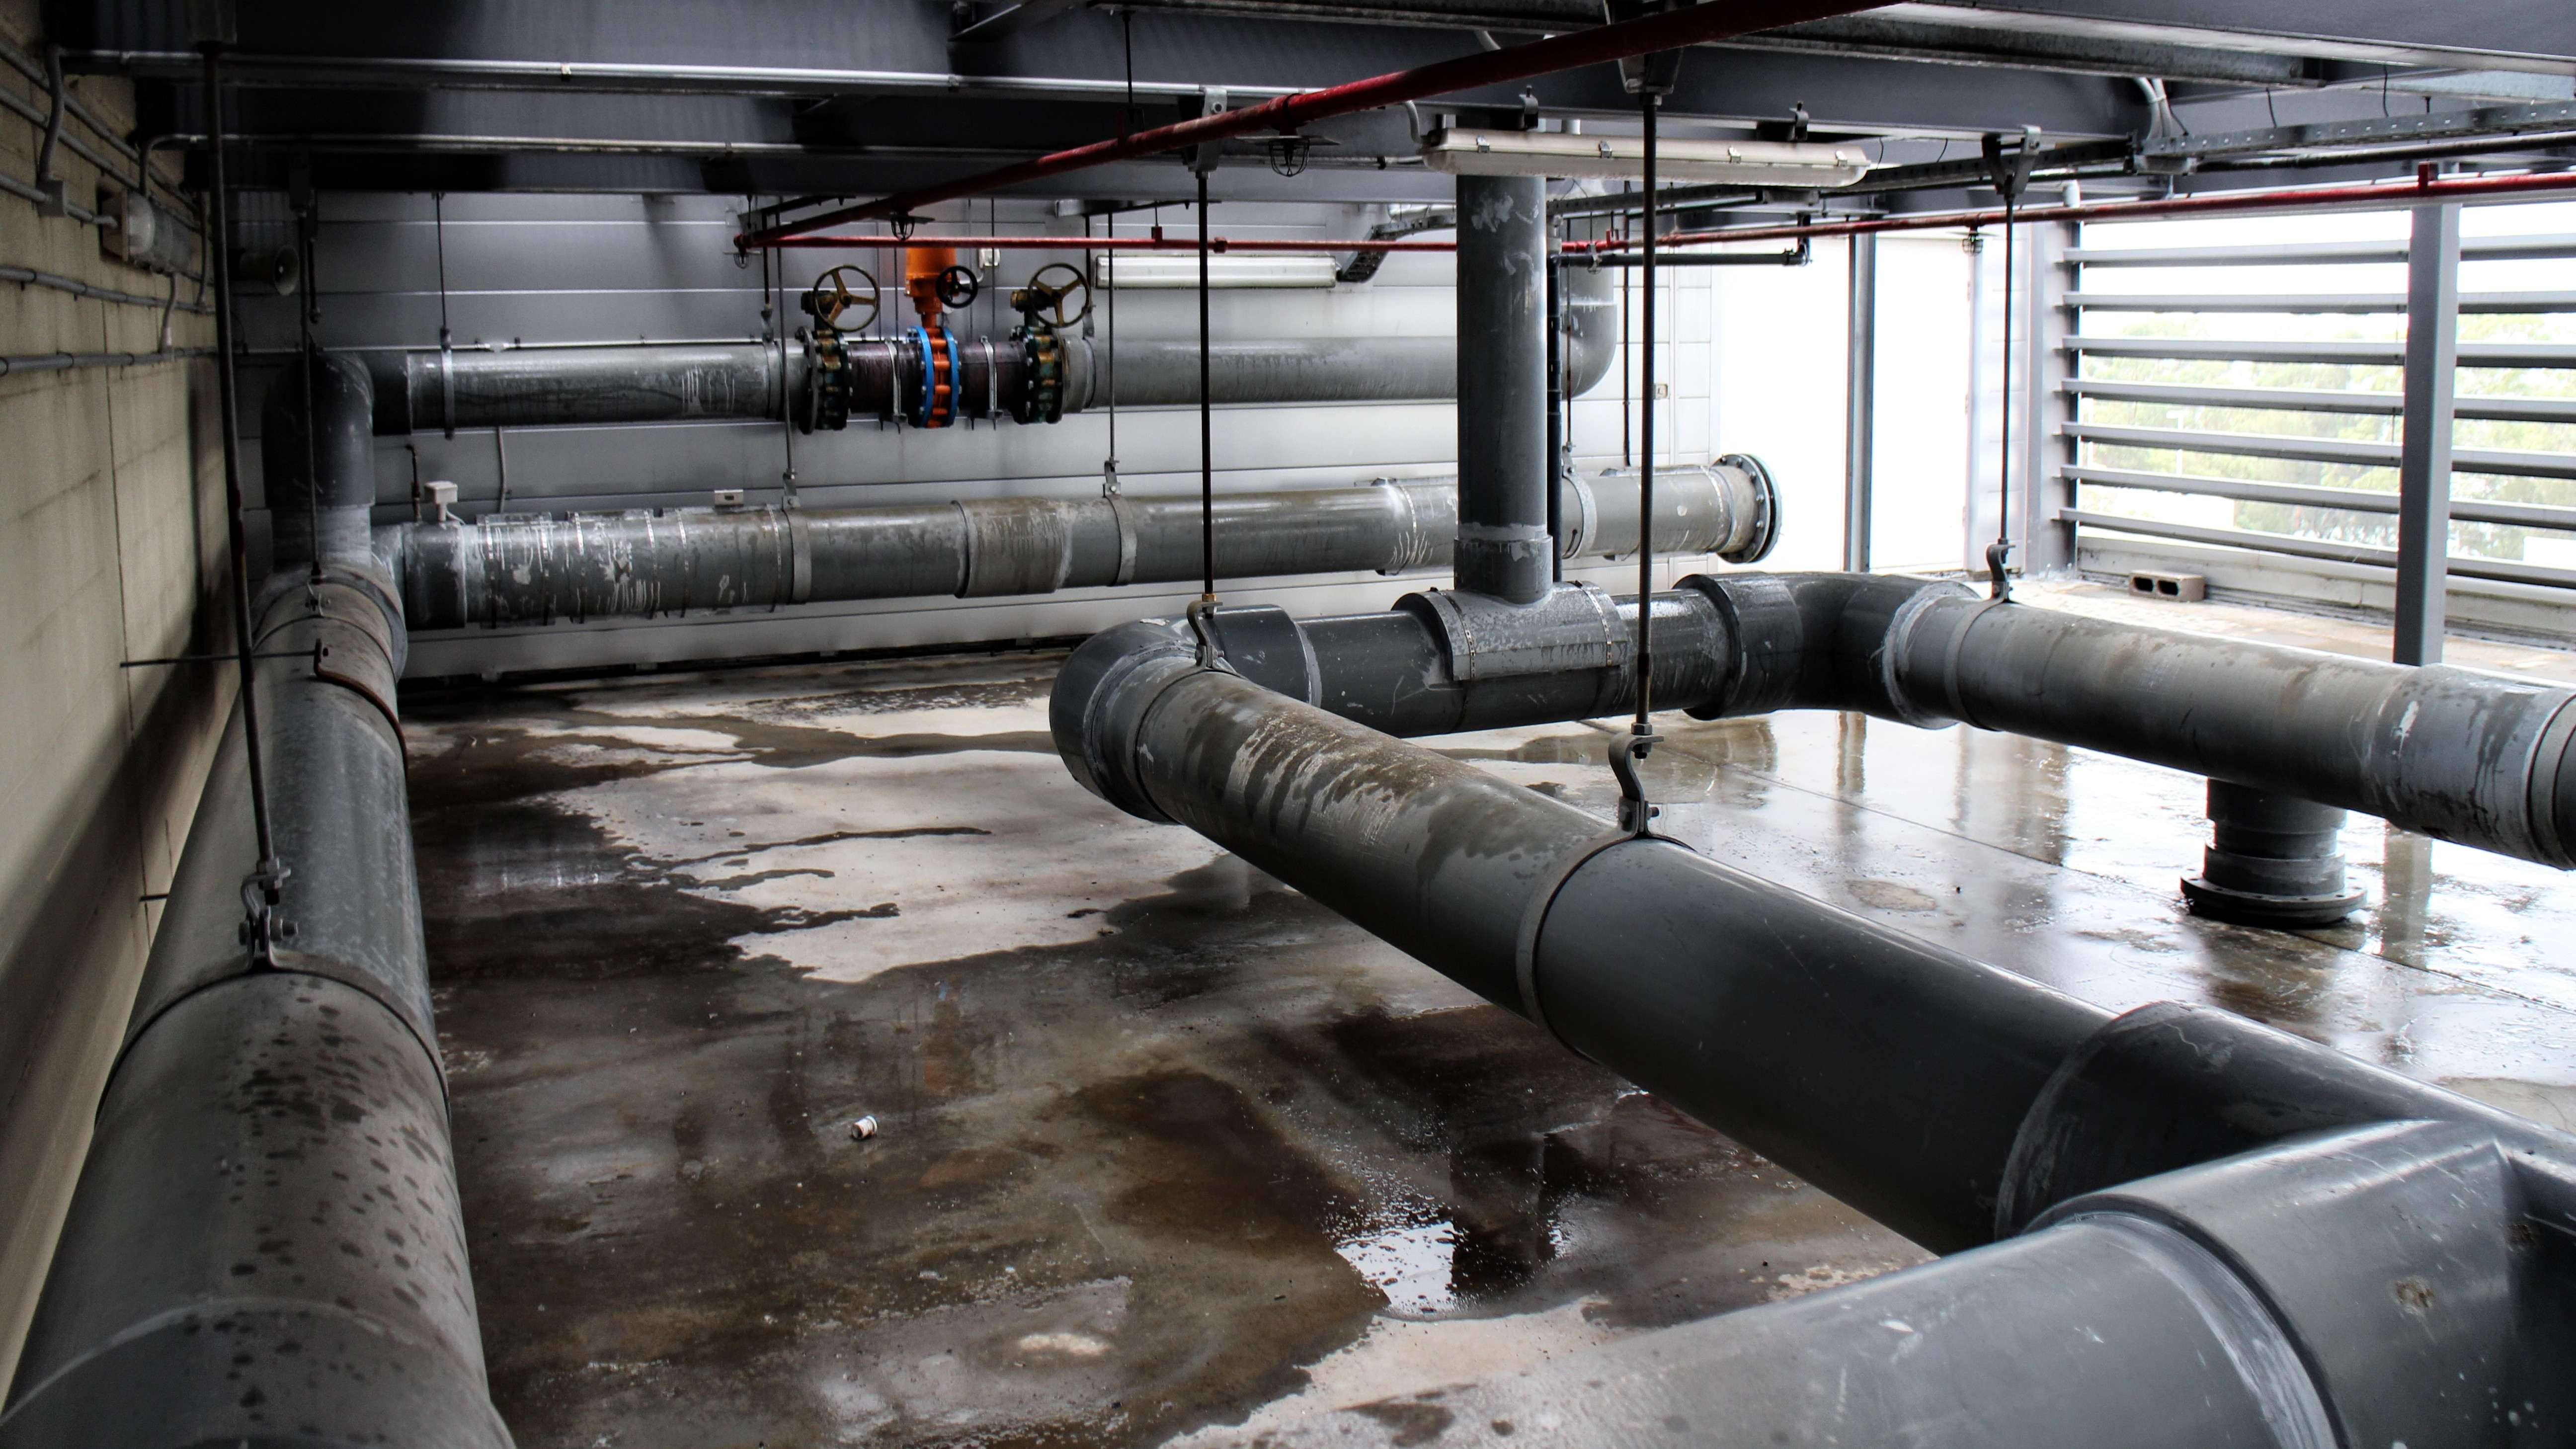
\includegraphics[width=\paperwidth]{img/pipes.jpg}}
  \begin{frame}[plain]
  \end{frame}
}

\begin{frame}
  \vfill
  {\huge Pipes \cmd{|}}\large
  \vfill
  A pipeline is a set of processes chained together by their standard streams, so that the output text of each process (\cmd{stdout}) is passed directly as input (\cmd{stdin}) to the next one.
  \vfill
  Example:
  \vfill
  \begin{itemize}
    \item \cmd{process1 | process2 | process3}
  \end{itemize}
  \vfill
  Processes are started in parallel and outputs are buffered.
  \vfill
  You can also redirect outputs to files:
  \vfill
  \begin{itemize}
    \item \cmd{echo "Hello world!" > hello.txt}
  \end{itemize}
  \vfill
\end{frame}

\begin{frame}
  \vfill
  {\Large\cmd{cat}\quad con\textbf{cat}tenate and print files on the standard output}
  \vfill
  \begin{itemize}
    \item \cmd{cat file1.txt file2.txt file3.txt}
    \item but more commonly just \cmd{cat file.txt} to take a quick look
  \end{itemize}
  \vfill
  {\Large\cmd{more} or \cmd{less}\quad can scroll through input}
  \vfill
  \begin{itemize}
    \item Remember that ``less is more,'' and use \cmd{less}
    \item \cmd{cat my_file.txt | less} is equivalent to \cmd{less myfile.txt}
  \end{itemize}
  \vfill
  {\Large\cmd{head} or \cmd{tail}\quad outputs the first or last part of files}
  \vfill
  \begin{itemize}
    \item\cmd{head my_big_data_file.csv} is useful to just check the headers
    \item\cmd{tail running_simulation.csv -f} will follow (\cmd{-f}) the file as it's updated
  \end{itemize}
  \vfill
\end{frame}

\begin{frame}
  \vfill
  {\Large Also useful:}
  \vfill
  \begin{itemize}
    \item\cmd{column data.csv -t -s,}\quad outputs a table (\cmd{-t}) using comma separator (\cmd{-s,})
    \item\cmd{cat data.csv | wc -l}\quad counts the number of lines in the file
  \end{itemize}
  \vfill
  {\Large Search and replace:}
  \vfill
  \begin{itemize}
    \item \cmd{grep}\quad find regular expressions in files
    \item \cmd{find -name *.png -exec convert \{\} \{\}.jpg \\;}\quad find files and act on them
    \item \cmd{sed -e 's/more/less/' unix_intro_slides.tex | grep less}\\edit files as text streams
  \end{itemize}
  \vfill
  {\Large Editors:}
  \vfill
  \begin{itemize}
    \item \cmd{vi}\quad modal editor --- exits with \cmd{:q}
    \item \cmd{nano}\quad as simple as it gets
  \end{itemize}
  \vfill
\end{frame}

\begin{frame}
  \vfill
  {\Large Network connections:}
  \vfill  
  \begin{itemize}
    \item \cmd{ssh}\quad connect to a server via Secure SHell
    \item \cmd{scp}\quad copy files over \texttt{ssh} connection
    \item \cmd{wget} and \cmd{curl}\quad download files over network
    \item \cmd{screen} and \cmd{tmux}\quad manage your sessions
  \end{itemize}
  \vfill  
  {\Large System info:}
  \vfill
  \begin{itemize}
    \item \cmd{top}/\cmd{htop}\quad manage your processes
    \item \cmd{free -h}\quad display free \emph{memory} in human readable format
    \item \cmd{df -h}\quad display free \emph{disk space} in human readable format
    \item \cmd{nproc}\quad display how many processors you have
  \end{itemize}
  \vfill
\end{frame}

\begin{frame}
  \vfill
  {\huge Other basic stuff, just for reference}
  \vfill
  \begin{itemize}
    \item \cmd{cp}\quad copy files
    \item \cmd{ln -s}\quad create a soft link
    \item \cmd{mkdir}\quad create a new directory
    \item \cmd{mv}\quad move files and/or rename them
    \item \cmd{rm -rf}\quad remove files and directories (\cmd{-r}) without prompting (\cmd{-f})
    \item \cmd{touch}\quad change the time stamp of the file, creating it if needed
  \end{itemize}
  \vfill
\end{frame}
